In this document, we propose to construct an approach to secure a serverless system using \textit{Distributed Information Flow Control}. For a system to be secure at the programming level, it is imperative that \textbf{confidentiality} and \textbf{integrity} is enforced. While confidentiality is described as the virtue of a system to protect it's sensitive data from being disclosed to unauthorized parties, where as integrity can be explained as the ability of a system to prevent an information from being manipulated or modified by unauthorized parties. Going forward, all the essential ideas will be elaborated in this section as follows: \ref{section:ServerlessComputing} introduces \textit{Serverless Computing}, where as \ref{section:InformationFlowControl} talks about the information flow control model. Furthermore, \ref{section:NonInterference} describes the phenomena of \textit{non-interference} in security, and \ref{section:TSNI} describes two types of information flow control enforcements, \textit{Termination Insensitive Non Interference} (TINI), and \textit{Termination Sensitive Non Interference} (TSNI). Here, TSNI is described formally. Finally, \ref{section:ExistingApproaches} discusses existing approaches that employ IFC to secure serverless systems.

\section{Serverless Computing}
\label{section:ServerlessComputing}
With the rise in usage of Cloud Computing, different architectures have been introduced by vendors over time, increasing efficiency, performance, and at the same time, decreasing the cost. In the early days, Infrastructure as a Service, or IaaS was prevalent, which provided virtual servers in the cloud. However they were still servers, with the difference being - the need to personally own the servers was not required anymore. Further, the concept of PaaS, or Platform as a Service was introduced, that delivered virtual application platforms, viz. JAVA Spring Boot, Python Flask, Node JS Express, etc. Here, the developers were no more responsible for maintaining the operating system. Nevertheless, packaging an application for deployment and  managing the scalability was still critical. Although after the introduction of container orchestration platforms such as Docker Swarm, Kubernets, etc. PaaS has started gaining more popularity.
%\footnote{B. Christner, “Docker Serverless,” 2017. [Online]. Available:
%	https://pt.slideshare.net/BrianChristner/docker-serverless?from\_action=save}


%\begin{wrapfigure}{r}{0.71\textwidth} %this figure will be at the right
	\begin{framed}
		\centering
		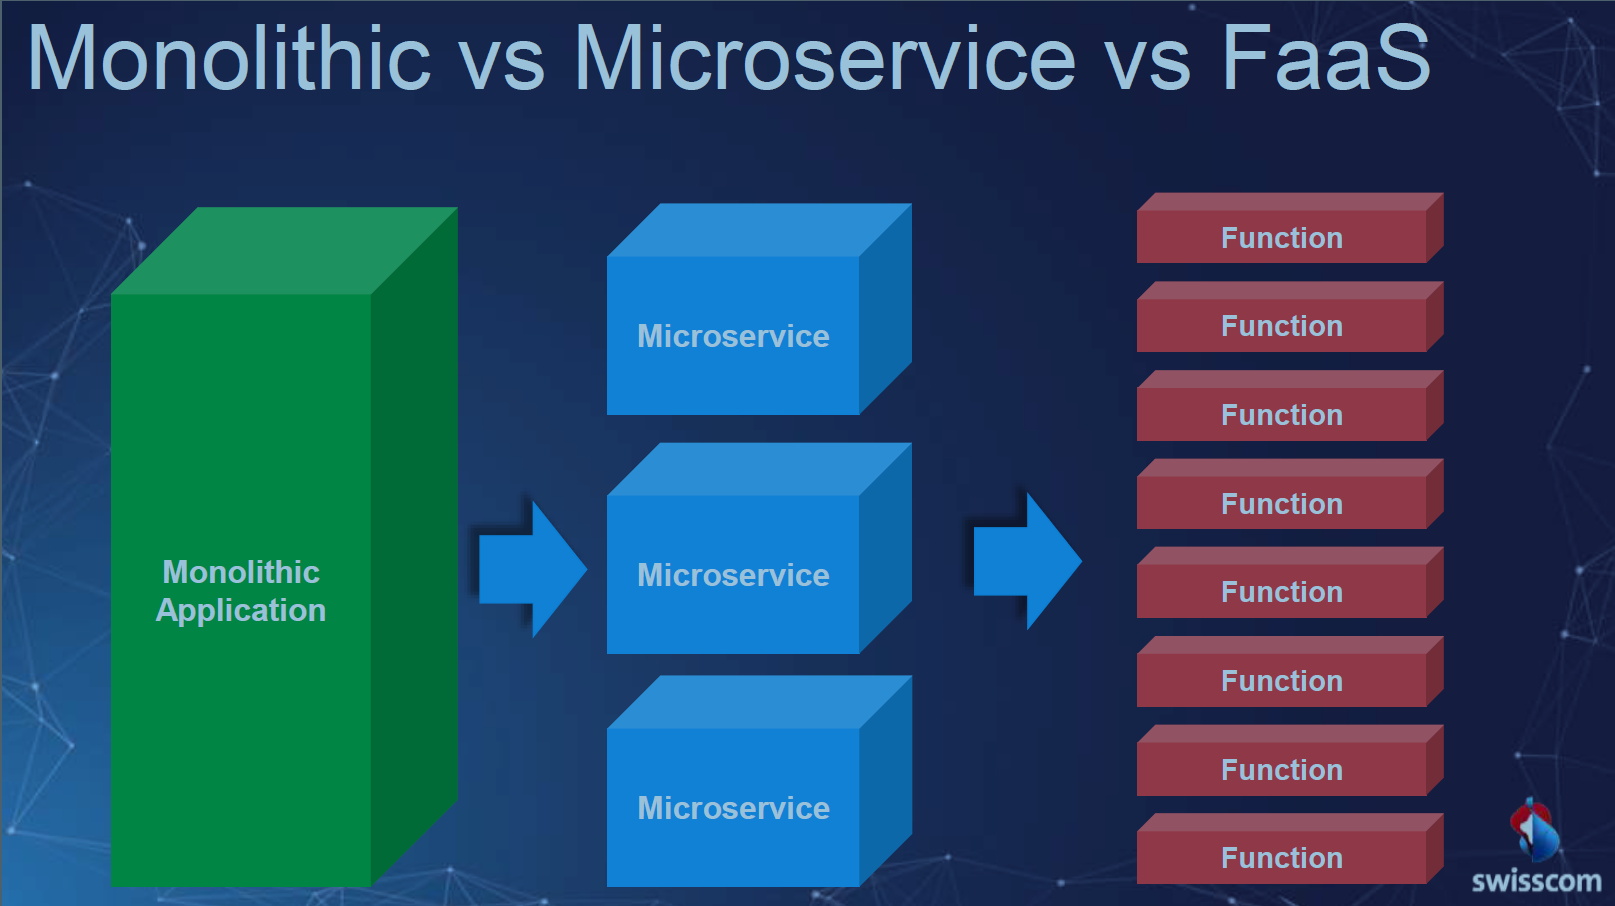
\includegraphics[width=\textwidth]{images/monoVSmicroVSfaas.png}
		\captionof{figure}{Graphical representation of the architectural difference between a Monolithic Application (IaaS), a Microservices-Based Application (PaaS), and Serverless (FaaS)
		}
		\label{fig:IaaSPaaSFaaS}
	\end{framed}
%\end{wrapfigure}


Finally, Functions as a Service (FaaS), or \textit{Serverless Computing} was introduced, which can intuitively be perceived as taking the resource abstraction to its logical \mbox{conclusion \footnotemark}. \addtocounter{footnote}{0} \footnotetext{S. Waterworth, “Introduction to Serverless Computing,” 2018.
https://www.instana.com/blog/introduction-to-serverless-computing/} It is needless to say that Serverless Computing still involves servers. However in this case, developers spend minimum time in maintaining or managing servers as compared to previous-generation architectures. Instead of accommodating a monolith application or a collection of microservices, Serverless architecture only contains a set of functions deployed individually. Figure~\ref{fig:IaaSPaaSFaaS} shows the contrast between the aforementioned architectures\footnote{B. Christner, “Docker Serverless,” 2017. https://pt.slideshare.net/BrianChristner/docker-serverless}.

\section{Information Flow Control}
\label{section:InformationFlowControl}
Information flow control, or IFC mainly focuses on building secure systems irrespective of the fact that the system might contain faults or bugs. It is difficult to build secure systems in the first place, as a single bug in any line of code may lead to security vulnerability. Therefore, it is not surprising to learn that in many cases, a simple bug has resulted in the disclosure of many sensitive information, such as personal identity, credit card numbers, etc.\footnote{L. H. Newman, “The Equifax Breach Was Entirely Preventable,” Wired, 2017. https://www.wired.com/story/equifax-breach-no-excuse}$^{,}$\footnote{Big data breach! Aadhaar software hack raises major security concerns, BusinessToday. https://www.businesstoday.in/current/economy-politics/aadhaar-software-hack-uidai-data-ghost-entries/story/282260.html}$^{,}$\footnote{T. Armerding, “The 18 biggest data breaches of the 21st century,” CSO Online, 2018. https://www.csoonline.com/article/2130877/the-biggest-data-breaches-of-the-21st-century.html}. As a result, there are a lot of strategies available currently that focuses on finding and fixing bugs such as SQL Injection, Temporary file races, Buffer overflows, Missing access checks, Format string bugs, Integer overflow, etc. However, it is important to note that most of these bugs require different methodologies in order to tackle them; and therefore, it has eventually become a battle between the attacker and security expert for who find the next bug in a system first. In case of the former, the system might be exploited and in case of the latter, the bug might be fixed, and the system made secure – until the next bug is discovered. As it can be observed, this approach to make the system secure does not appear to be practical, as it can eventually turn out to be risky and costly, since declaring a system completely bug-free is not possible.\footnote{SteelKiwi Inc, “Is There Such a Thing As Bug-free Software?,” Hackernoon, 2018. https://hackernoon.com/is-there-such-a-thing-as-bug-free-software-320cd862af17.}$^{,}$\footnote{R. Varshneya, “There’s No Such Thing as a Bug-Free App,” Entrepreneur India, 2015. https://www.entrepreneur.com/article/251742}$^{,}$\footnote{Allen, “The Myth of ‘Bug Free’ Software,” BetaBreakers, 2016. https://www.betabreakers.com/the-myth-of-bug-free-software} Let us contemplate a small illustration to support our argument – consider a simple eCommerce website that sells books online. The web-application is built under different layers of abstraction, as shown in the Figure~\ref{fig:eCommerceArchitecture}. The web application itself enforces some kind of security policy that restricts one user to access the credit-card or address information of any other user. Going a level down, the web server, such as Apache could have its own security policy that ensures which web browser can make what http requests, etc. Going deeper, the operating system might have some enforcements to protect different Windows/UNIX users from one another. In the same vein, the hardware could be providing some mechanism to protect the kernel from application code, etc. As we can intuit, for the whole system to be secure, the code at every abstraction layer must be correct, or bug-free. However, as we are aware, all these layers combined comprise of millions of lines worth of code, and therefore, occurrence of one or more bugs anywhere up the stack is inevitable. Consequently, it can be said that the strategy of securing a system by the means of fixing a bug is practically impossible. This implies that securing a system completely via fixing all the discovered bugs is impossible. Nevertheless, via Information Flow Control, it is indeed possible to build a secure system despite the existence of bugs in the code.

\begin{figure}[h]
	\begin{framed}
		\centering
		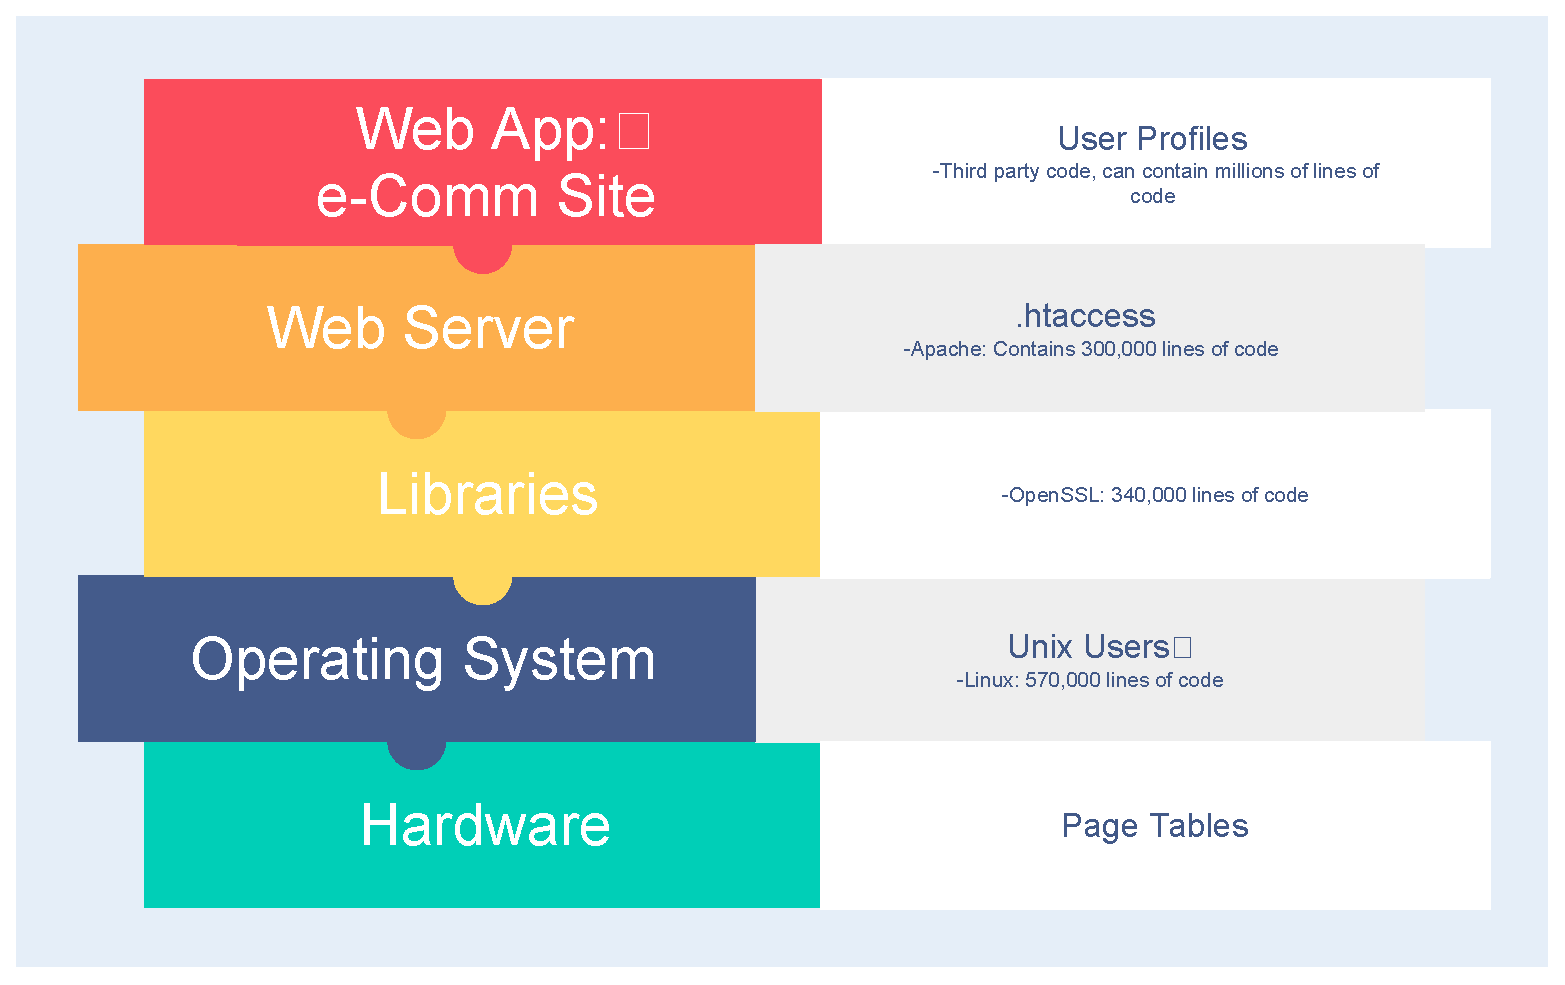
\includegraphics[width=\textwidth]{images/architectures.eps}
		\caption{A software architecture diagram for a simple e-commerce web application.}
		\label{fig:eCommerceArchitecture}
	\end{framed}
\end{figure}

Let us now take a step back and realise the fact that ensuring the security of a system is, in varying degrees, dependent on the data, rather than the code. As an instance, in the example shown in above (Figure~\ref{fig:eCommerceArchitecture}), a user wouldn’t want their credit-card data to be unauthorizedly accessed or sent to another location by an attacker. Assuming we can \textit{control and monitor all these data movements in a system}, and so long as the data remain secure, it is of no concern to supervise what is being done to the data by the application code. Trying to secure a system through this approach achieves the goal to secure the system without caring about the existing bugs in the system. Furthermore, enforcing IFC at lower abstraction level in an application ensures that the application remains secure in all the above abstraction levels. IFC is conceptually a simple idea: A label is associated with every piece of data in a system, and this label usually applies to data at all different levels of abstraction, ranging from \textit{hardware} to the \textit{application data}. Additionally, this label follows the data as it moves around through the system, and ultimately this label specifies what can happen to the data. For instance, it can make sure that the copy a user's credit-card number cannot be sent to an attacker's website. If this idea of Information Flow Control is implemented appropriately, the hope is that a system could be made secure without concerning ourselves with numerous existing bugs in the system.

The information flow model is an extension of the state machine model that constantly monitors the situation of a system to restrain it from entering an insecure state. A system that supports a state machine model must have the potential states of its process inspected in all the circumstances to confirm that they are controlled. Under the benchmarks laid down by the model, a system that boots up in a secure state and preserves the security of any transaction throughout itself shall, at all times, be in a secure state. Consequently, the information flow model consists of state transitions, objects and lattice states that regulate data flow policy. The fundamental purpose of information flow model is to restrict the flow of insecure and unauthorized data in any direction throughout the system. The exchange of data across different systems could be regulated using \textit{guards}, that can be employed by the information flow model. \textit{Flume} is a popular decentralized information flow control (DIFC)\cite{Myers2000} model and system ``\textit{that applies at the granularity of operating system processes and standard OS abstractions (e.g., pipes and file descriptors)}''\cite{Krohn2007}. 

\section{Non Interference}
\label{section:NonInterference}
Non-Interference in this research refers to the protection of the secret (\textit{high-sensitive}) part of the memory from an attacker who can observe the public (\textit{low-sensitive}) part of the memory\cite{Sabelfeld2005}. It is a policy that imposes an attacker to not be able to make a distinction between two computations from their outputs, in case they vary only in their secret inputs. It was first proposed in 1982\cite{Gougen1982}, and is a further development of the information flow model built to assure that the objects and subjects at different security level do not interfere with each other. In this context, the subjects may be applications, system users, or processes, while objects can be processes, bits of data, programs or documents. Additionally, \textit{information flow monitors} is an evolved technique that dynamically enforces noninterference. As one would expect, dynamic monitors enforce non interference differently for different instances of the execution of process under observation. This is because the information control flow of a program can be different for different input values, thus making the program secure for some set of values, while declaring it insecure for others. This is in contrast with static monitors, that will completely declare a program insecure, even if it becomes insecure for a very small range of input values. Therefore, it can be said that dynamic monitors allows analysis in further details, as compared to static monitors, as it is in the beginning of the execution of a dynamic monitor, when the assignment of security levels to the variables takes place. Moreover, the assigned security levels do not change throughout the execution. Adding to this, there also exists several \textit{hybrid} monitors \cite{Shroff2007, Russo2010, Guernic2007} that combine both static and dynamic methodologies.\par
It must, however be noted that even dynamic monitors are prone to produce false positives. Hence, there is a need to construct improved monitors that allow multiple \textit{paths}. These challenges were scoped by Khakpour and Skandylas in their research \cite{Khakpour2018} where a new approach was proposed that, at some designated checkpoints, supervises a program written in a subset of Java based on boolean supervisory controller synthesis \cite{BERTHIER201446} to construct a hybrid monitor that, to avoid future leakages, applies suitable countermeasures in checkpoints by forecasting security breaches. This approach is supported by a tool implemented in OCAML and uses SOOT to analyze the program at the java bytecode level.

\section{Termination Sensitive Non Interference}
\label{section:TSNI}
Information Flow Control (IFC) \cite{Denning1976, Hedin2011} based security techniques could be an optimistic approach to tackle the security problem in Serverless Applications. However, a security policy known as Termination Insensitive Non-Interference (TINI) have been implemented by most of the previous implementations. Intuitively, it is ensured by TINI that a program's non secret outputs are not allowed to expose any secrets stored in the system. On the other hand, the fact that the system ceased to generate outputs could be utilized to deduce some part of the secret. This channel, also known as the \textit{termination-channel} is usually neglected as it just leaks one bit. Furthermore, Askarov et al. have claimed that it might leak more than just a bit \cite{Askarov2008}. However, for Serverless Applications, even the leakage of a single bit might be dangerous, as these are highly scalable and triggering parallel computations, each leaking one bit could be performed to access the secure data. Another strong security policy, called as Termination Sensitive Non Interference (TSNI) \cite{Sabelfeld2001} could be enforced that eliminates the termination channel. Let us formally define TSNI followed by observing an example:\par
\medskip
%\begin{minipage}{\textwidth}
	\begin{mdframed}[linewidth = 0.05cm, backgroundcolor=blue!20, nobreak=true]
		\noindent Consider a Program \textbf{P}:
		\begin{framed}
			\lstinputlisting[language=Octave]{codes/tsni.txt}
		\end{framed}
		\noindent \textbf{We define some notations as:}\par
		{cH} \tab Input Channel \par \medskip
		\textbf{P} \tab The above program \par \medskip
		$\mu$ \tab Memory \par \medskip
		$State<P,\mu>$ \tab A program state. \par \medskip
		$terminating(P, \mu, I)$ \tab If the $State<P,\mu>$ is executed with input $I$, \tab \tab \tab then it terminates. \par \medskip
		$I_{1} = _{L} I_{2}$ \tab both $I_{1}$ and $I_{2}$ belong to the same security \tab \tab \tab level \textbf{L}, which can either be public or \tab \tab \tab confidential. \par \medskip
		\noindent $State<P,\mu>$ is TSNI  $\forall I_{1} \& I_{2} \iff$
		\begin{framed}
			\begin{equation} \label{eq:TSNI}
			I_{1} = _{L} I_{2} \land terminating(P, \mu, I_{1}) \Longrightarrow terminating(P, \mu, I_{2})
			\end{equation}
		\end{framed}
		\noindent \textbf{TSNI either converges or diverges $\forall$ I $\equiv$ L}
	\end{mdframed}
%\end{minipage}
\medskip
As an example, for the program \textbf{P} above, let us consider a \textbf{State} $<P, \mu>$ where two inputs $I_{1}$ \& $I_{2}$ belong to the same channel \textbf{cH} and are of the same security level, which is \textit{confidential}. Therefore, $I_{1} = _{L} I_{2}$, where \textit{L} is a \textit{confidential} security level. Let us now consider the values of $I_{1}$ \& $I_{2}$: \par
\begin{itemize}
	\item $I_{1} = [cH: 0]$
	\item $I_{2} = [cH: 1]$
\end{itemize}
It is known that in program P, an input where h>0 will result in an infinite loop, whereas any input that does not satisfy the above condition will terminate. Therefore, based on the input values assigned to $I_{1}$ \& $I_{2}$, we can say that:
\begin{equation} \label{eq:NoTSNI}
I_{1} = _{L} I_{2} \land terminating(P, \mu, I_{1}) \Longrightarrow \neg terminating(P, \mu, I_{2})
\end{equation}
As it can be clearly observed, the Equation \ref{eq:NoTSNI} above contradicts the definition of TSNI in Equation \ref{eq:TSNI} in Page \pageref{eq:TSNI}. Hence, it can be stated that the \textbf{State} $<P, \mu>$ does not satisfy TSNI.

\section{Existing Approaches}
\label{section:ExistingApproaches}
\textit{Google Scholar}\footnote{Google Scholar - https://scholar.google.co.in/}, which could be considered as one of the biggest search portal for scientific literature was used to look for other existing approaches that uses Information Flow Control to secure a Serverless system. Following were the set of keywords used:
\begin{center}
	\begin{mdframed}[frametitle=Keywords Used, linewidth = 0.05cm, backgroundcolor=blue!20, nobreak=true]
		\textit{(tsni \textbf{OR} tini \textbf{OR} "termination sensitive non interference" \textbf{OR} "termination insensitive non interference" \textbf{OR} "information flow control" \textbf{OR} "distributed information flow control" \textbf{OR} difc \textbf{OR} ifc) \textbf{AND} (serverless \textbf{OR} "serverless computing")}
	\end{mdframed}
\end{center}
Based on the above keyword-combination, we could only find one relevant research that uses Information Flow Control to secure a Serverless Computing system. This approach, proposed by Alpernas et al. \cite{Alpernas2018} aims to secure a serverless computing system by ensuring confidentiality via enforcing termination sensitive non interference (TSNI). The tool developed by the authors, called as Trapeze Framework \footnote{Trapeze Framework - https://github.com/kalevalp/trapeze} is written in JavaScript and at the moment, only supports the node.js runtime. The author claims that TSNI enforcement is essential in case of serverless computing, since the termination channel, which usually leaks just a bit cannot be disregarded; as the attacker can amplify the termination channel by executing many parallel computations, each leaking one bit.